%%%%%%%%%%%%%%%%%%%%%%%%%%%%%%%%%%%%%%%%%%%%%%
% Header
\documentclass[11pt]{report}
\usepackage[english]{babel}
\usepackage[utf8x]{inputenc}
\PassOptionsToPackage{hyphens}{url}\usepackage{hyperref}
\usepackage{graphicx}
\usepackage{fullpage}
\usepackage{nicefrac}
\usepackage[lastexercise]{exercise}
\usepackage[dvipsnames]{xcolor}
\usepackage{amsmath}
\usepackage{enumitem} 


\usepackage{minted}
\makeatletter
\AtBeginEnvironment{minted}{\dontdofcolorbox}
\def\dontdofcolorbox{\renewcommand\fcolorbox[4][]{##4}}
\makeatother


\setlength{\parindent}{0cm}

\renewcommand{\ExerciseHeader}{\large\textbf{\ExerciseName~\ExerciseHeaderNB} - \textbf{\ExerciseTitle}\medskip}

\renewcommand{\ExePartHeader}{\medskip\textbf{\ExePartName\ExePartHeaderNB\ExePartHeaderTitle\medskip}}

\begin{document}

%%%%%%%%%%%%%%%%%%%%%%%%%%%%%%%%%%%%%%%%%%%%%
\subsubsection*{Introduction to Computer Programming}
\subsection*{\Large Exercises -- Week 8. Computational Modelling and Documentation}

\subsection*{\Large Part 1. Expressing algorithms}

\begin{Exercise}[title=Building Flow Diagrams of Algorithms (Essential)]\label{Ex:flow_diagrams}

For each question you should draw a flow chart to represent the process needed to solve the question. You may find it helpful to write out some or all of the steps on chronological order first. 

% \begin{enumerate}[label=(\roman*)]
%     \item Read the real-world problem
%     \item Identify the steps in chronological order
%     \item Assign a type to each step (shape used to represent it)
%     \item Draw chart
%     \item Confirm the chart is correct by carefully reviewing the steps.
% \end{enumerate}

You may use software to create the lists and diagrams or write/draw them by hand. 

  \Question{Convert temperature from Fahrenheit ($^{\circ}$F) to Celsius ($^{\circ}$C) using the formula $$C = \frac{5}{9}\times(F-32)$$ where $C$=temperature in ($^{\circ}$C) and $F$ = temperature in ($^{\circ}$F).}
  
  \Question{A student will pass the year if the average score for 5 units is 40\% or above. Write a program that can be used to determine if a student passes or fails the year. 
    }

  \Question{A bank account has an interest rate of 3\%. The interest accrued is calculated at the end of each year. The initial deposit is £200. At the start of each subsequent year, £100 is added the bank account. Display the interest accrued at the end of each year. }

  \Question{A digital thermostat checks the current temperature read by a sensor and compares it to a preset temperature. The heating is switched:
  \begin{itemize}
      \item ON if temperature lower than the preset temperature
      \item OFF if temperature higher than, or same as, the preset temperature
  \end{itemize}
  Determine whether the heating should be ON or OFF using the present temperature and the current temperature, and display the outcome.}

  
\end{Exercise}


\begin{Exercise}[title=Building more Flow Diagrams of Algorithms (Advanced)]\label{Ex:flow_diagrams_advanced}

  \Question{Determine the largest in a sequence of numbers and display the outcome.}
  
  \Question{Display the first 10 Fibonacci numbers.}
  
  \Question{Check if a word is in a sentence. }

%   \Question{Sort 3 different numbers a,b,c in descending order using steps:
%   \begin{enumerate}[label=(\roman*)]
%     \item Enter values of a,b,c ({\it Input})
%     \item Check if a $>$ b ({\it Decision})
%     \item Whatever the outcome (True or False), next check if a $>$ c ({\it Decision})
%     \item From the outcome of steps 2 and 3, you will either know the order at this point and should display it, or you will require one further check to see if b $>$ c. ({\it Decision})
%     \item Display the order if you haven't done so already. ({\it Output})
%     \end{enumerate}
%     }
  
\end{Exercise}




\subsection*{\Large Part 2. Computational Models}

\begin{Exercise}[title= Translating Algorithms to Code (Essential)]

  \Question{For each of the questions in Exercise \ref{Ex:flow_diagrams}, write a program to execute the steps you have drawn up in the flow diagram.}
  
  \Question{Translate the flow diagram of  Euclid's algorithm for computing the greatest common divisor (GCD) [also known as the greatest common factor (GCF) or highest common factor (HCF)] of two positive integers (Figure \ref{fig:euclid}) to a program.}

  \Question{Translate the flow diagram of an algorithm to generate a 12 by 12 multiplication table (Figure \ref{fig:12x12}). }

\end{Exercise}

\begin{figure}[!h]
        \centering
        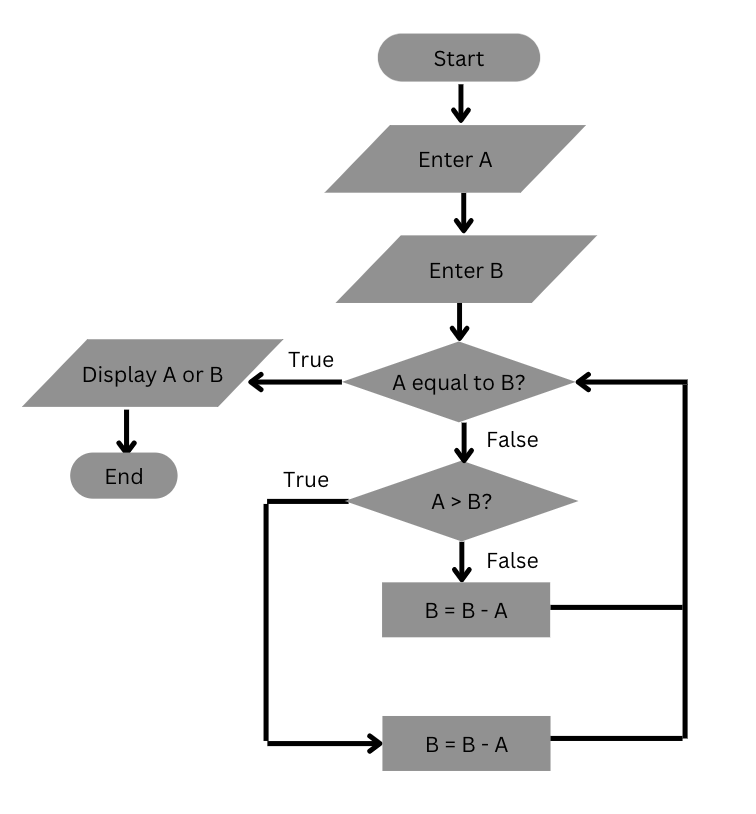
\includegraphics[height=10cm]{img/Ex3_2.png}
        \caption{Euclid's algorithm for computing the greatest common divisor (GCD).}
        \label{fig:euclid}
\end{figure}

\begin{figure}[!h]
        \centering
        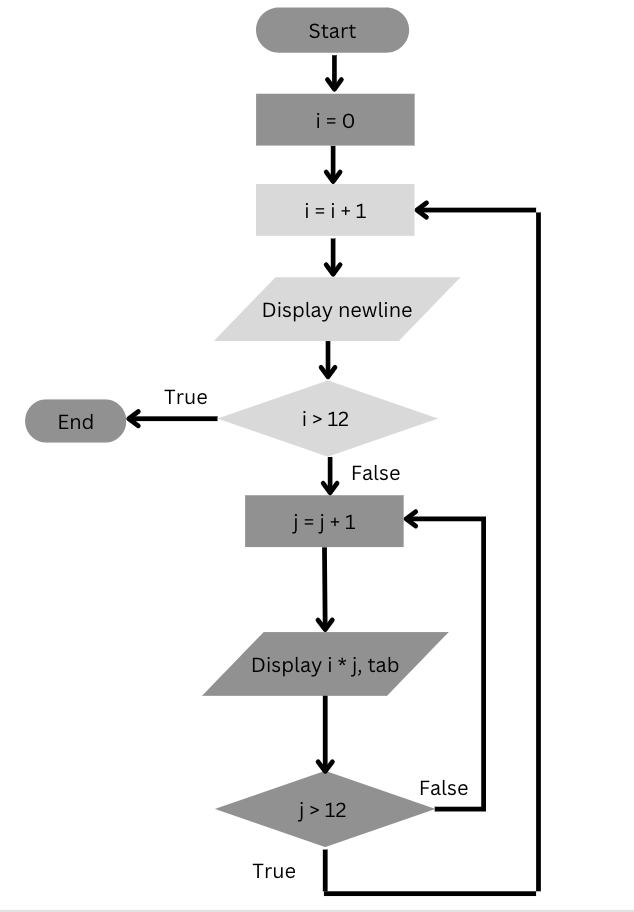
\includegraphics[height=10cm]{img/Ex3_3.png}
        \caption{An algorithm to generate a 12 by 12 multiplication table.}
        \label{fig:12x12}
\end{figure}


\begin{Exercise}[title= Translating Algorithms to Code (Advanced)]

  \Question{For each of the questions in Exercise \ref{Ex:flow_diagrams_advanced}, write a program to execute the steps you have drawn up in the flow diagram.}
  
  \Question{Translate the flow diagram of an algorithm to sort 3 different numbers a,b,c in descending order.}
  

\end{Exercise}


\end{document}